\section{Learning Paradigms and Terminology}
In describing the learning paradigms and the terminology we must keep in mind an objective: to be able to generalize the concepts observed.
\begin{definition}[Neural Network]
    A neural network is a sorted triple $(N,V,w)$ with two sets $N,V$ and a function w, where N is the set of neurons and V is a set ${(i,j)|i,j\in\mathbb{N}}$ whose elements are connections between neurons. The function $w: V \longrightarrow \mathbb{R}$ defines the weights where $w((i,j))$, the weight between neuron i and j, is shortened $w_{i,j}$
\end{definition}
The data flow is more than just a graph: data enters a neuron where it follows three steps:
\begin{description}
    \item[Propagation function] Often a weighted sum, transforms outputs of other neurons to net input
    \item[Activation function] Transforms net input and sometimes old activation to new activation
    \item[Output function] Often the identity function, transforms activation to output for other neurons
\end{description}
\begin{definition}[Propagation function and network input]
    Let $I = \left\{ i_{1}, \ldots,i_{n} \right\}$ be the set of neurons such that $\forall z\in \left\{ 1, \ldots, n \right\} : \exists w_{i_z,j}$. Then the network input of j, called $net_j$, is calculated by the propagation function $f_prop$ as follows
    \[ 
        net_j = f_prop(o_{i_1},\ldots, o_{i_n}, w_{i_1,j} \ldots w_{i_n,j}) 
    \]
    Most often the $f_prop$ is the weighted sum and operates on previous layers' output
\end{definition}
\begin{definition}[Threshold value]
    Let j be a neuron. The threshold value $\Theta_j$ is uniquely assigned to j and marks the position of the maximum gradient value of the avtivation function.
\end{definition}

\begin{definition}[Activation state/ activation in general] Let j be a neuron. The activation state $a_j$, in short activation, is explicitly assigned to j, indicates the extent of the neurons activity and results from the activation function.
    \[ 
        a_j(t) = f_act(net_j(t), a_j(t-1), \Theta_j) 
    \]
    
\end{definition}
Most often, the output function is the identity function. Unlike the other variables within the neural network the activation functions is often defined globally for all neurons, or at least for a set of neurons and only the threshold values are different for each neurons. The following are commong activation functions:
\begin{figure}[htbp]
    \centering
    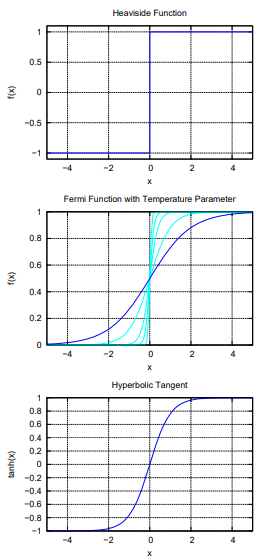
\includegraphics[width=8cm]{Learning Paradigms/activation_functions.png}
\end{figure}
\newpage
\begin{definition}[Output function]
    Let j be a neuron. The output function
    \[ 
        f_out(a_j)= o_j 
    \]
    calculates the output value of $o_j$ of the neuron j from its avtivation state $a_j$.
\end{definition}
    Generally the output function is defined globally. Often this function is the identity function $f_out(a_j) = a_j,\; o_j = a_j$
\begin{definition}[Bias neuron]
    A bias neuron is a neuron whose output value is always 1. It is used to represent neuron biases as connection weights, which enables any weight training algorithm to train the biases at the same time.
\end{definition}
\subsection{Network Topologies}
\subsubsection{Feed-Forward}
The Feed-forward network topology has input nodes, hidden/processing nodes, and output nodes. Most often layers are fully connected. They can be varied adding shortcuts between input and output cutting through the network while in the simplest topology each neuron is only connected to neurons of the adjacent layer.
\begin{figure}[htbp]
    \hspace*{-2cm}
    \centering
    \begin{subfigure}{8cm}
      \centering
      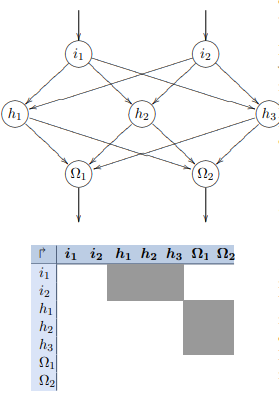
\includegraphics[width=6cm]{Learning Paradigms/simplest_ffnn.png}
      \caption{Simplest Feed-forward NN}
      \label{fig:sub1}
    \end{subfigure}%
    \begin{subfigure}{8cm}
      \centering
      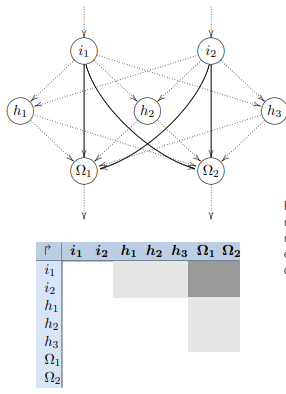
\includegraphics[width =6cm]{Learning Paradigms/shortcut_ffnn.png}
      \caption{Feed-forward NN with shortcuts}
      \label{fig:sub2}
    \end{subfigure}
    \caption{Feed-forward topologies}
    \label{fig:feedforward}
    \end{figure}
\subsubsection{Recurrent}
By recurrence in the context of NN we mean the process of a neuron influencing itself by any means or by any connection.
In recurrent NN it's not as clear what neurons are the outputs. The use and impact of recurrence in neural networks is extremely complex and is still being researched. Recurrence can be of three types: direct (self loop), indirect, lateral.
\begin{figure}[htbp]
    \centering
    \begin{subfigure}{6cm}
      \centering
      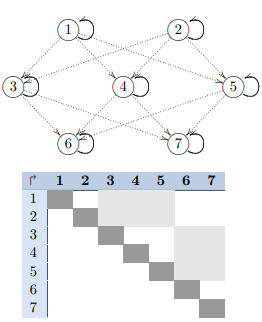
\includegraphics[width=5cm]{Learning Paradigms/direct_recurrence.png}
      \caption{Direct recurrence}
      \label{fig:sub1}
    \end{subfigure}%
    \begin{subfigure}{6cm}
      \centering
      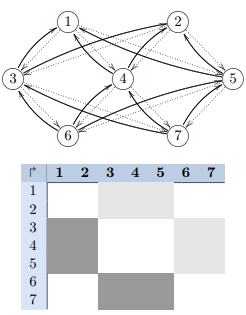
\includegraphics[width =5cm]{Learning Paradigms/indirect_recurrence.png}
      \caption{Indirect recurrence}
      \label{fig:sub2}
    \end{subfigure}
    \begin{subfigure}{6cm}
        \centering
        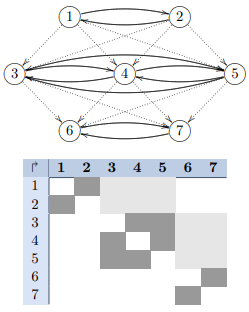
\includegraphics[width =5cm]{Learning Paradigms/lateral_recurrence.png}
        \caption{Lateral recurrence}
        \label{fig:sub3}
      \end{subfigure}
    \caption{Recurrence in NN}
    \label{fig:recurrence}
    \end{figure}
\subsection{Order of activation}
To describe the order of activation we have two classes:
\begin{description}
    \item[Synchronous activation]: all neurons change their values synchronously ( they simultaneusly calculate network input, activation and output, and pass them on). The syncronous activation corresponds closest to its biology counterpart but not particularly effective for real world hardware, especially if used on Feed-forward NN.
    \item[Asynchronous activation]: here, the neurons do not change their values simultaneusly but at different points of time. For this, there exist different orderds:
    \begin{description}
        \item[Random Order] a random neuron i is chosen and its $net_i, a_i, o_i$ are updated. For n neurons a cycle is the n-fold execution of this step. Some neurons might be updated more than once and other never.
        \item[Random Permutation] in this case each neuron is chosen exactly once but in a random order, during one cycle.
        \item[Topological Order] the neurons are updated during one cycle and according to a fixed order. The order is defined by network topology. 
    \end{description} 
\end{description}
\begin{definition}[Input Vector]
    A network with n input neurons needs n inputs $x_{1}, \ldots,x_{n}$. They are considered as input vecotr $ x = (x_{1}, \ldots,x_{n})$. As a consequence the input dimension is referred to as n.
\end{definition}
\begin{definition}[Output Vector]
    A network with m output neurons provides m outputs $y_{1}, \ldots,y_{n}$. They are considered as output vecotr $ y = (y_{1}, \ldots,y_{n})$. As a consequence the output dimension is referred to as m.
\end{definition}

\subsection*{Learnin paradigms}
How do we act on a NN to improve its ability towards generalization? There are at least 7 actions that we can take:
\begin{itemize}
    \item developing new connections
    \item deleting existing connections
    \item changing connecting weights
    \item changing the threshold values of neurons
    \item varying one or more of the three neuron functions
    \item developing new neurons
    \item deleting existing neurons (and of course connections)
\end{itemize}
\begin{definition}[Training set]
    A training set (named P) is a set of training patterns $p_{1}, \ldots,p_{n}$, which we use to train our neural net. 
\end{definition}
Two questions quickly arise when thinking about the network's ability to learn 
\begin{itemize}
    \item How do NNs learn?
    \item When do NNs stop learning?
\end{itemize}
There are three essential paradigms of learning by presenting the differences between their training set.
Unsupervised learning is the biologically most plausible method, but is not suitable for all problems. Only the input patterns are given; the network tries to identify similar patterns and to classify them into similar categories.
\begin{definition}[Unsupervised Learning]
    The training set only consists of input patterns, the network tries by itself to detect similarities and to generate pattern classes.
\end{definition}
In reinforcement learning the network receives a logical or a real value after completion of a sequence, which defines whether the result is right or wrong. Intuitively it is clear that this procedure should be more effective than unsupervised learning since the network receives specific criteria for problem-solving.
\begin{definition}[Reinforcement Learning]
    The training set consists of input patterns, after completion of a sequence a value is returned to the network indicating whether the result was right or wrong and, possibly, how right or wrong it was.
\end{definition}
In supervised learning the training set consists of input patterns as well as their correct results in the form of the precise activation of all output neurons. Thus, for each training set that is fed into the network the output, for instance, can directly be compared with the correct solution and the network weights can be changed according to their difference.
\begin{definition}[Supervised Learning]
    The training set consists of input patterns with correct results so that the network a precise error vector can be returned.
\end{definition}
\begin{definition}[Offline learning]
    Several training patterns are entered into the network at once, the errors are accumulated and it learns for all patterns at the same time.
\end{definition}
\begin{definition}[Online learning]
    The network learns directly from the errors of each training sample.
\end{definition}
\subsection{Learning curve and error measurement}
\begin{definition}[Training patterns]
    A training pattern is an input vector p with the components $p_{1}, \ldots,p_{n}$ whose desired output is known. By entering the training pattern into the network we receive an output that can be compared with the teaching input, which is the desired output. The set of training patterns is called P. It contains a finite number of ordered pair (p, t) of training patterns with corresponding desired output.
\end{definition}
\begin{definition}[Teaching Input]
    Let j be an output neuron. The teaching input $t_j$ is the desired and correct value j should output after the input of a certain training pattern. Analogously to the vector p the teaching inputs $t_{1}, \ldots,t_{n}$ of the neurons can also be combined into a vector $t$. $t$ always refers to a specific training pattern $p$ and is, as already mentioned, contained in the set P of the training patterns.
\end{definition}
\begin{definition}[Error Vector]
    For serveral output neurons $\Omega_{1}, \ldots,\Omega_{n}$ the difference between output vector and teaching input under a training input p
    \[ 
        E_p = \begin{bmatrix}
            t_1-y_1 \\
            \vdots\\
            t_n-y_n
        \end{bmatrix} 
    \]is referred to as error vector. 
\end{definition}
The learning curve indicates the progress of the error, which can be determined in various ways.
\begin{definition}[Specific Error]
    The specific error $Err_p$ is based on a single training sample, which means it is generated online.\\
    Additionally, the Root Mean Square and the Euclidean Distance are often used.
\end{definition}
\begin{definition}[Total Error]
    The total error $Err$ is based on all training samples, that means it is generated offline.
\end{definition}
The Hebbian rule is the basis for most of the more complicated learnig rules. In its original idea we can think of it as a formal way to express a simple concept: strengthen more all the strong bonds and loosen even further all the loose bonds
\begin{definition}[Hebbian rule]
    If neuron j receives an input from neuron i and if both neurons are strongly active at the same time, then increase the weight $w_{i,j}$
    $\Delta w_{i,j} = \eta o_i a_j$
\end{definition}
\begin{definition}[Generalized Hebbian rule]
    The generalized form of the Hebbian rule only specifies the proportionality of the change in weight to the product of two undefined functions, but with defined values
    \[ 
        \Delta w_{ij} = \eta h(o_i,w_{i,j})g(a_j,t_j)
    \]
\end{definition}
With our newly acquired understanding of learning paradigms and field terminology we can give a better definition of Perceptron
\begin{definition}[Perceptron]
    The perceptron is a feedforward network insipired by the human eye. It has at least one trainable weight layer and every neuron layer is completely connected to the following layer.
\end{definition}
\subsection{The delta rule as a gradient base learning strategy}
In this subsection we deviate from the binary threshold value as activation function because at least for back-propagation of error we need a differntiable or even a semi-linear activation function. Suppose that we have a singlelayer perceptron with randomly set weights which we want to teach a function by means of training samples. The set of these training samples is called P. It contains the pairs (p,t) of the training sample p and its teaching input t. Now our learning target will certainly be that for all training samples the output y of the network is approximately the desired output t. This means that we first have to understand the total error Err as a function of the weights.
\begin{definition}[Error Function]
    The Error function
    \[ 
        Err : W \longrightarrow \mathbb{R} 
    \]regards the set of weights W as a vector and maps the values onto the normalized output error.
\end{definition}
So we try to decrease or to minimize the error by simply tweaking the weights by calculating the gradient $\nabla Err(W)$ or the error function Err(W)
\[ 
    \Delta W \sim -\nabla Err(W) 
\]Due to this relation there is a proportionality constant $\eta$ for which the equality holds:
\[ 
    \Delta W = -\eta \nabla Err(W) 
\]We rewrite the gradient of the error function according to all weights as an usual partial derivative. Thus, we tweak every single weight and observe the error function changes:
\begin{align*}
    \Delta w_{i,\Omega} &= -\eta \frac{\partial Err(W)}{\partial w_{i,\Omega}}\\
    &=\sum_{p\in P}{-\eta \frac{\partial Err_p(W)}{\partial w_{i,\Omega}}}
\end{align*}
\begin{definition}[Delta rule]
    If we determine that the function h of the Hebbian theory only provides the output $o_i$ of the predecessor neuron i and if the function g is the difference between the desired activation $t_\Omega$ and the actual activation $a_\Omega$, we will receive the delta rule, also known as Widrow-Hoff rule:
    \[ 
        \Delta w_{i,\Omega} = \eta \cdot o_i \cdot (t_\Omega -a_\Omega)= \eta o_i \delta_\Omega
    \]
\end{definition}
\subsection{SLP limitations and MLP}
If we try to find a SLP that can correctly learn the logic function XOR we can quickly see that the problem is impossible. This is because the SLP model is only capable of representing linearly separable data. Furthermore we can see that as the dimension grows fewer and fewer binary functions are linearly separable.  A multilayer perceptron represents an universal function approximator which is proven by the Theorem of Cybenko. 
\begin{definition}[Multilayer perceptron]
    Perceptrons with more than one layer of variably weighted connections are refered to as multilayer perceptrons (MLP).
\end{definition}
\subsection{Convergence and Complexity of the Perceptron}
The problem of fitting a half-space or a linear separator consists of n labeled examples $x_{1}, \ldots,x_{n}$ in d-dimensional space. Each example has label $+1$ or $-1$. The task is to find a d-dimensional vector w, if one exists, and a threshold t such that
\begin{align*}
    w\cdot x_i > t \text{ for each } x_i \text{ labeled }+1\\
    w\cdot x_i < t \text{ for each } x_i \text{ labeled }-1
\end{align*}
A vector-threshold pair (w,t) satisfying the inequalities is called a linear separator. We begin with a technical modification adding an extra coordinate to each $x_i, w$, writing $\hat{x}_i=(x_i,1)$ and $\hat{w} =(w,-t)$. Suppose $l_i$ is the $\pm 1$ label on $x_i$. Then, the inequalities can be rewritten as 
\[ 
    (\hat{w} \cdot \hat{x})l_i > 0 \quad 1 \leq i \leq n 
\]
Adding the extra coordinate increased the dimension by 1 but now the separator contains the origin.
\begin{theorem}
    If there is a $w^*$ satisfying $(w^*\cdot x_i)l_i\geq 1$ for all i, then the Perceptron algorithm finds a solution w with $(w\cdot x_i)l_i >0$ for all i in at most $r^2\absolute{w^*}^2$ updates where $r = \max_{i}{\absolute{x_i}}$
    \begin{proof}
        Let $w^*$ satisfy the if condition of the theorem. We will keep track of two quantities, $w^Tw^*$ and $\absolute{w}^2$. Each update increases $w^Tw^*$ by at least 1.
        \[ 
            (w+x_il_i)^Tw^* = w^Tw^* + x_i^Tl_iw^* \geq w^Tw^*+1
        \]
        On each update, $\absolute{w}^2$ increases by at most $r^2$
        \[ 
            (w+x_il_i)^T(w+x_il_i) =\absolute{w}^2+ 2x_i^Tl_iw+\absolute{x_il_i}^2 \leq \absolute{w}^2 +\absolute{x_i}^2 \leq \absolute{w}^2+r^2 
        \]
        where the middle inequality comes from the fact that an update is only performed on an $x_i$ when $x_i^Tl_iw\leq 0$. If the perceptron algorithm makes m updates, then $w^Tw^* \geq m$ and $\absolute{w}^2 \leq mr^2$ or equivalently $\absolute{w}\absolute{w^*}\geq m$ and $\absolute{w} \leq r \sqrt{m}$. Then
        \begin{align*}
            m \leq& \absolute{w}\absolute{w^*} \\
            \frac{m}{\absolute{w^*}} \leq& \absolute{w}\\
            \frac{m}{\absolute{w^*}} \leq & r \sqrt{m} \\
            \sqrt{m} \leq & r\absolute{w^*}\\
            m \leq & r^2\absolute{w^*}^2
        \end{align*}
    \end{proof}
\end{theorem}

\subsection{Kernel Functions}
In the case that the input data is not linearly separable we can add an extra dimension by employing kernel functions, practice often referred to as "kernel trick". With adding extra dimension we mean adding computed features.\\
Suppose you have a function k, called a "kernel", over pairs of data points such that for some function $\varphi: \mathbb{R}^d \longrightarrow \mathbb{R}^N$, we have $K(x,x') = \varphi(x)^T\varphi(x')$.\\ Key point: after the transformation $\varphi$ I need to go back to the perceptron algorithm on the new data.  The kernel functions will assist me in computing a value after $\varphi$.  Issue: we now must run the perceptron algorithm on the new data, the new weights are linear combinations of the $\varphi(\vec{x_i})$
\[ 
    w^T = \sum_{i=1}^{n}{c_i\varphi(x_i)}
\]all we need is the value of $\varphi$ on $x_i$
\[ 
    w^T\varphi(x_j)= \sum_{i=1}^{n}{c_i\varphi(x_i)^T\varphi(x_j)}
\]
To compute what we want we just need the kernel function
\[ 
    k(x_i,x_j) = \varphi(x_i)^T\varphi (x_j)
\]
\begin{theorem}
    Suppose $k_1$ and $k_2$ are kernel functions. Then
    \begin{itemize}
        \item For any constant $c\geq 0 \quad ck_1$ is a legal kernel. In fact, for any scalar function f the function $k_3(x,x') = f(x)f(x')k_1(x,x')$ is a legal kernel
        \item The sum $k_1+k_2$ is a legal kernel
        \item The product $k_1k_2$ is a legal kernel
    \end{itemize}
\end{theorem}
\begin{lemma}
    A matrix K is a kernel matrix (there is an embedding $\varphi$ such that $k(x_i,x_j) = \varphi(x_i)^T\varphi (x_j)$) if and only if K is positive semi-definite.
    \begin{proof}
        If K is positive semi-definite then it can be expressed as $K = BB^T$. Define $\varphi(x_i)$ to be the i-th row of B. Then $k(x_i,x_j) = \varphi(x_i)^T\varphi (x_j)$. Conversely, if there is an embedding $\varphi$ such that $k(x_i,x_j) = \varphi(x_i)^T\varphi (x_j)$, then using the $\varphi(x_i)$ for the rows of a matrix B, we have that $K=BB^T$ and so K is positive semi-definite.
    \end{proof} 
\end{lemma} 
\textbf{Intuition:} if we know how $\varphi$ operates on the examples we know enough about it.\\Notice that the kernel matrix is always defined as a dot product. A particular example of a kernel is the Gaussian kernel $ k(x,y) = e^{-c\absolute{x-y}^2}$ which is defined by applying the rules to define a kernel infinitely many times.\\
We need to find the kernel ourselves (also part of the elements of the kernel can be learned with examples). To find the kernel we need to understand a metric which differntiates our classes of data and capture it, encapsulate it, through a kernel function to project the differences and highlight them allowing for linear separability